\documentclass[aps,prl,twocolumn,superscriptaddress]{revtex4-1}
\usepackage{graphicx}  % this is the up-to-date package for all figures
\usepackage{amssymb}   % for math
\usepackage{verbatim}  % for the comment environment
\usepackage{color}
\usepackage{subcaption} % for subcaptions on side-by-side figures
\usepackage{float}	% allows use of 'H' command
%\usepackage{hyperref}	% needed to add hyperlinks
%\hypersetup{
%  colorlinks=true,
%  linkcolor=blue,
%  filecolor=magenta,
%  urlcolor=cyan,
%}
\bibliographystyle{apsrev}


% these are some custom control of the page size and margins
% \topmargin= 0.2in  % these 1st two may be needed for some computers
% \textheight=8.75in
\textwidth=6.5in
%\oddsidemargin=0cm
%\evensidemargin=0cm

% this is where the actual document itself (rather than control statements) begins:

\begin{document}



\title{Transient Mapping}


\author{Daichi Hiramatsu}
\author{Corey Mutnik}
\email{dhiramat@hawaii.edu}
\email{cmutnik@hawaii.edu}
\affiliation{Department of Physics \& Astronomy, \\
University of Hawaii at Manoa,\\
2505 Correa Rd, Honolulu, HI, 96822, USA}
\altaffiliation{Observational Astronomy 301}



	      % \section is used to start a new one with a heading
\begin{abstract}

\end{abstract}

\maketitle    


\section{Data Collection}
$l^{II}=202^{\circ}$...
$b^{II}=\pm5$
\begin{table}[H]
	\begin{tabular}{ | c | c | c | c | c | } \hline
		& $b=$ (0) & $b=$ (0) & $b=$ (1) & $b=$ (1) \\
		& min & max & min & max \\ \hline \hline
		RA (no offset) & 93$^{\circ}$ & +108$^{\circ}$ & +102$^{\circ}$ & +117$^{\circ}$  \\ \hline
		Dec (no offset) & -20$^{\circ}$ & +8$^{\circ}$ & -15$^{\circ}$ & +12$^{\circ}$ \\ \hline
		RA (offset) & +93$^{\circ}$ & +108$^{\circ}$ & +102$^{\circ}$ & +117$^{\circ}$ \\ \hline
		Dec (offset) & -20$^{\circ}$ & +8$^{\circ}$ & -15$^{\circ}$ & +12$^{\circ}$ \\ \hline
	\end{tabular}
\end{table}

\section{Data Reduction}

\begin{itemize}
	\item{} Sorted data by going through 1deg x 1deg FOV
	\item{} Identify stars as most variable
	\item{} Run LS
	\item{} Discuss how we established uncertainty in period - how this propagates to distance calculations
	\item{} How are we going to determine distance - discuss PL-relation
\end{itemize}

\subsection{What JT Did For Newly Sorted/Reduced Data}

\begin{figure}[H]
 \centering
 %\caption{prob(f)}
 \textbf{Sorting Pattern}\par\medskip
 	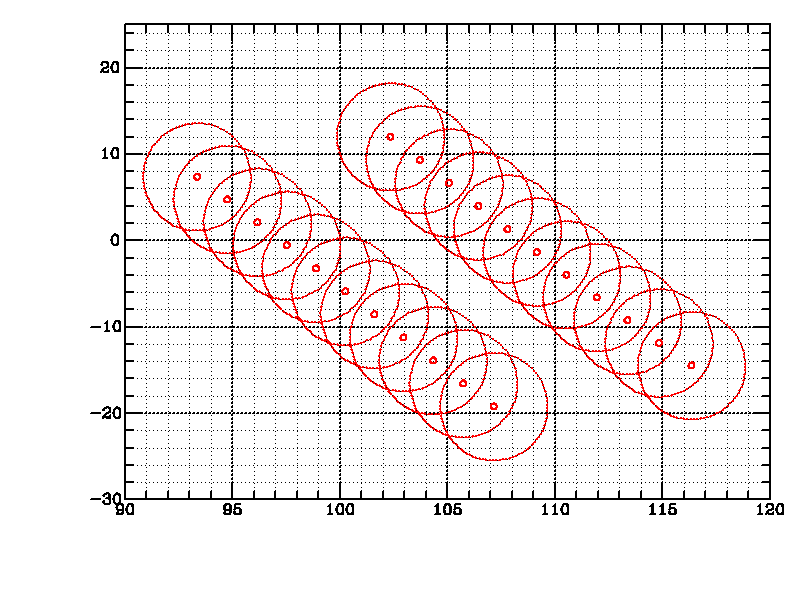
\includegraphics[width=3.35in]{figures/fromJT/sortedFOV.png}
 \caption{\it \small{Stars were grouped in the pattern shown (down the collected observations)}}
 \label{fig:sortpat}
\end{figure}

\begin{itemize}
 \item{} split observations into 1 $deg^2$ chunks
 \item{} isolated groups s.t. each one is a star with 12 or more obs
 \item{} $--$ more than 12 detections to be a star
 \item{} $--$ any sq deg that has more than one star
 \item{} this reduced 1300 $deg^2$ observation data down to ~300
 \item{} before variability params: 1531417 stars in field
 \item{} for variability parameters
 \item{} $--$ log(average(upper quartile)) - log(average(lower quartile))
 \item{} $--$ expect variation to go at .2* mag (from sqrt noise)...so subtract .2mag to get the logritmic statistic
 \item{} sorted biggest (most variable?) to smallest (least variable?)
 \item{} ran LS on 80,000 most variable stars, rather than full star groupings (over 1million)
\end{itemize}



\subsection{LS}

\begin{itemize}
 \item{} major aliasing at 1 day and 0.5 day periods
 \item{} things that fall at at -50 (in Figure~\ref{fig:quartiles}) means that those are VERY probably variable stars
 \item{} roughly \_\_\_\_\_ stars fell at -50 in Figure~\ref{fig:quartiles}
 \item{} 80,000 stars tested for variability
 \item{} other stars (outside of 80000) are statistically unlikely to be variable
\end{itemize}

\begin{figure}[H]
 \centering
 %\caption{prob(f)}
 \textbf{prob(f)}\par\medskip
 	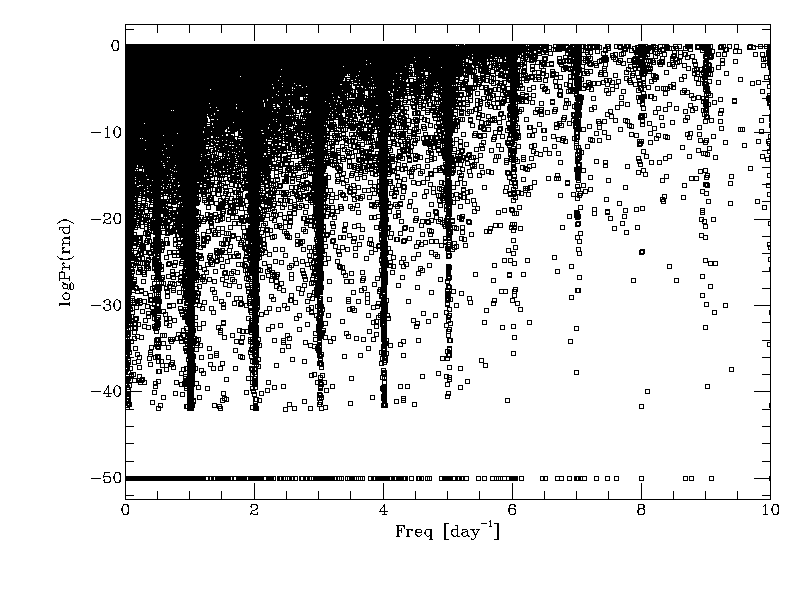
\includegraphics[width=3.35in]{figures/fromJT/probf.png}
 \caption{\it \small{prob(f) of 80,000, most variable, stars LS was run on}}
 \label{fig:quartiles}
\end{figure}




\section{Analysis}

\subsection{Pan-STARRS Comparison}
\begin{itemize}
	\item{} download Pan-STARRS data (finished)
	\item{} compare generated variable star list to PS RA and Dec
	\item{} validate observed variable stars
	\item{} Determine if PS parameters are worth anything (are candidates actually RR Lyraes)
\end{itemize}

\begin{figure}[H]
 \centering
 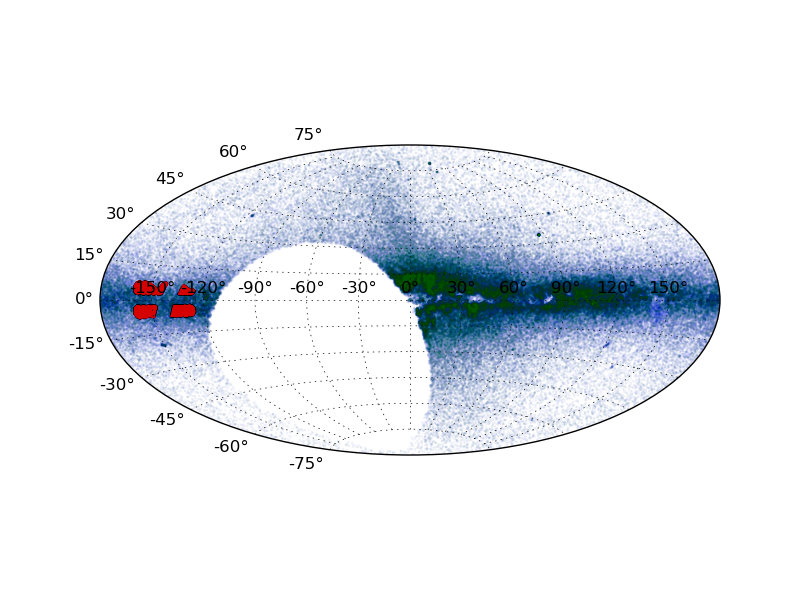
\includegraphics[width=3.35in]{figures/aitoff/Obs_PS_lsum_aitoff_map.png}
 \caption{\it \small{Aitoff projection of observed and PS RR Lyrae candidates.  Blue are candidates from PS that >= 0.05, green are PS candidates that >= 0.2., observed data in red.}}%
 \label{fig:aitoff_nosimbad}
\end{figure}

\subsection{Simbad Completeness}
\begin{itemize}
	\item{} Pull established RR list from Simbad
	\item{} Pull other variable data from simbad, too
	\item{} Compare list of observed RR to catalogs
	\item{} Is anyone actually reading this outline, this bullet point serves no purpose
	\item{} Wow, its sad how little Jeff did since class began (especially after JT gave him the code to do it a month ago) - 6 obs x 4 nights = January-April work period haha
	\item{} Establish completeness with Simbad
\end{itemize}


\iffalse
\begin{figure}[h!]
 \centering
 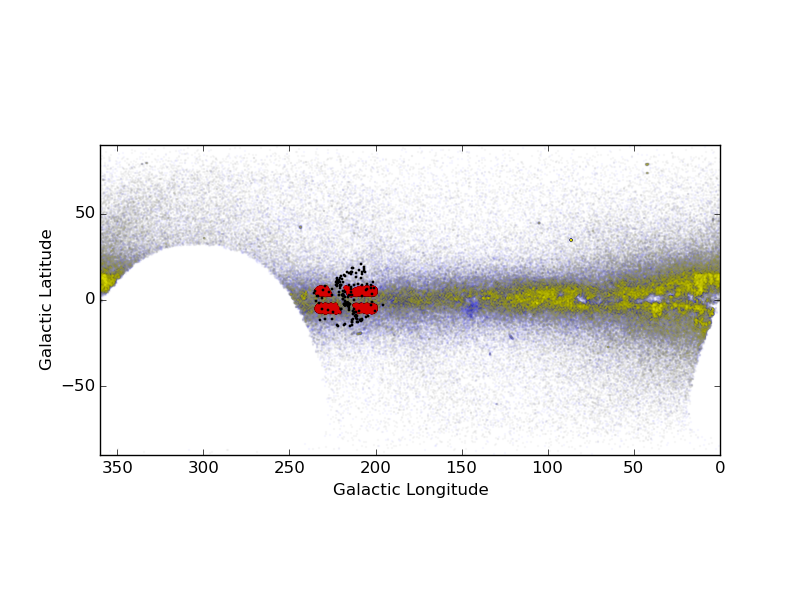
\includegraphics[width=3.35in]{figures/aitoff/simbad_alpha_is_1.png}
 \caption{\it \small{Aitoff projection of observed and PS RR Lyrae candidates.  Blue are candidates from PS that >= 0.05, yellow are PS candidates that >= 0.2., observed data in red, simbad in black.}}%
 \label{fig:aitoff_map_simbad}
\end{figure}
\begin{figure}[h!]
 \centering
 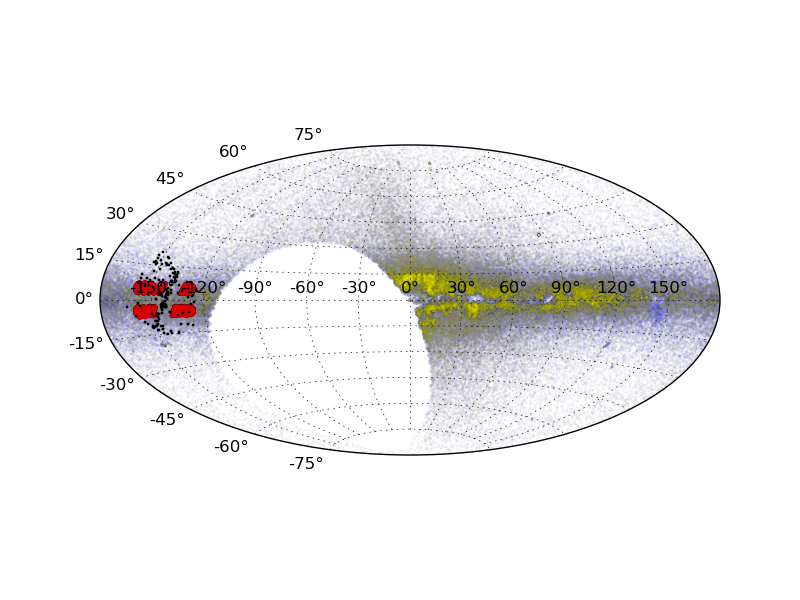
\includegraphics[width=3.35in]{figures/aitoff/Obs_PS_sim_lsum_aitoff_map.png}
 \caption{\it \small{Aitoff projection of observed and PS RR Lyrae candidates.  Blue are candidates from PS that >= 0.05, yellow are PS candidates that >= 0.2., observed data in red, simbad in black.}}%
 \label{fig:aitoff_simbad}
\end{figure}
\fi

%\clearpage

\begin{figure}[h!]
\centering
\begin{subfigure}{.5\textwidth}
  \centering
  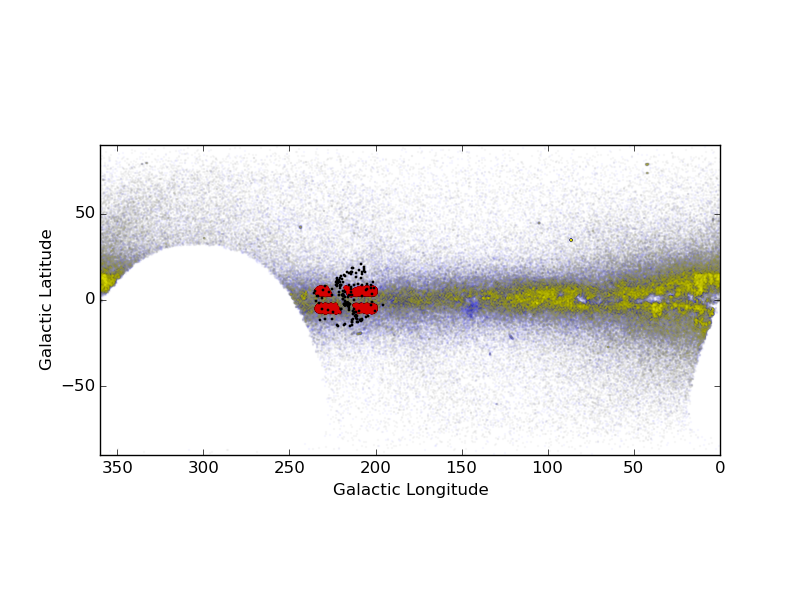
\includegraphics[width=1\linewidth]{figures/aitoff/simbad_alpha_is_1.png}
  \caption{\it \small{Aitoff map.}}
  \label{fig:aitoff_map_simbad}
\end{subfigure}%
\begin{subfigure}{.5\textwidth}
  \centering
  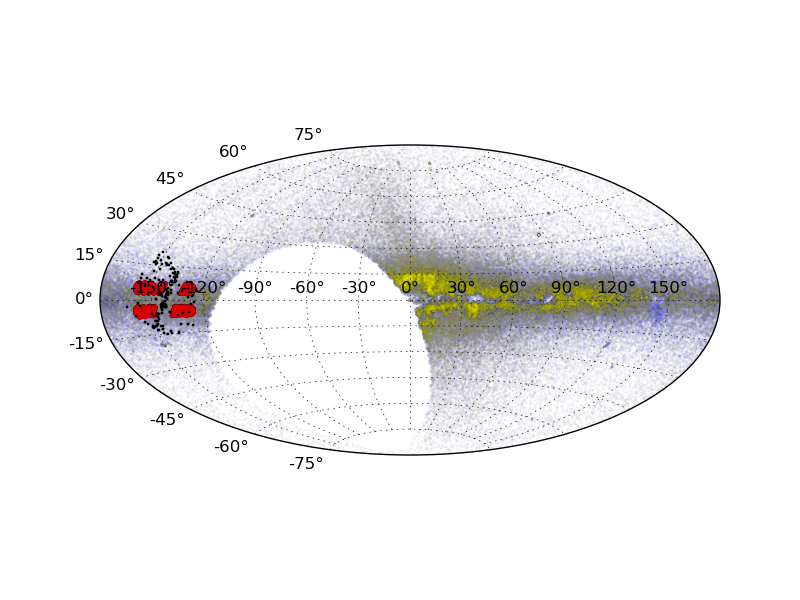
\includegraphics[width=1\linewidth]{figures/aitoff/Obs_PS_sim_lsum_aitoff_map.png}
 \caption{\it \small{Aitoff projection}}%
 \label{fig:aitoff_projection_simbad}
\end{subfigure}
\caption{\it \small{Aitoff projection of observed and PS RR Lyrae candidates.  Blue are candidates from PS that >= 0.05, yellow are PS candidates that >= 0.2., observed data in red, simbad in black.}}
\label{fig:aitoff_simbad}
\end{figure}



\subsection{3D map galaxy - var. stars}

\begin{itemize}
	\item{} Use gri data to identify variable stars
	\item{} Use Period-Luminosity relationship to get distance
	\item{} Map 3D spatial distribution
	\item{} Determine deviation of variable stars from model
	\item{} Variations arise from non-gravitational effects
	\item{} Figure out dark matter distribution
\end{itemize}





\section{Confirm accelerated expansion - Super Novea}
\begin{itemize}
	\item{} use PanStarrs data to identify supernova locations
\end{itemize}




%\begin{table}[h!]
%\label{data}
%\begin{center}
%\begin{tabular}{|c|c|c|c|} 
%\hline
%n  & Predicted $E_n$  & Simulated $E_n$    & Fractional Error \\
%\hline\hline
%0  & $\frac{1}{2}\hbar\omega$ & $0.500000035\hbar\omega$ & $7.0\times10^{-8}$\\
%\hline
%\end{tabular}
%\caption{\it\small{Comparison of simulated and predicted eigenvalues}}
%\end{center}
%\end{table}




\setlength{\parindent}{0cm}

\begin{thebibliography}{99}  % the trailing 99 controls some obscure format--just use

%\bibitem{Sch_eq} Weisstein, Eric W. ``Schr\"{o}dinger Equation."

\end{thebibliography}


\end{document}

